\section{Theorie}
\begin{figure}[h]
    \centering
    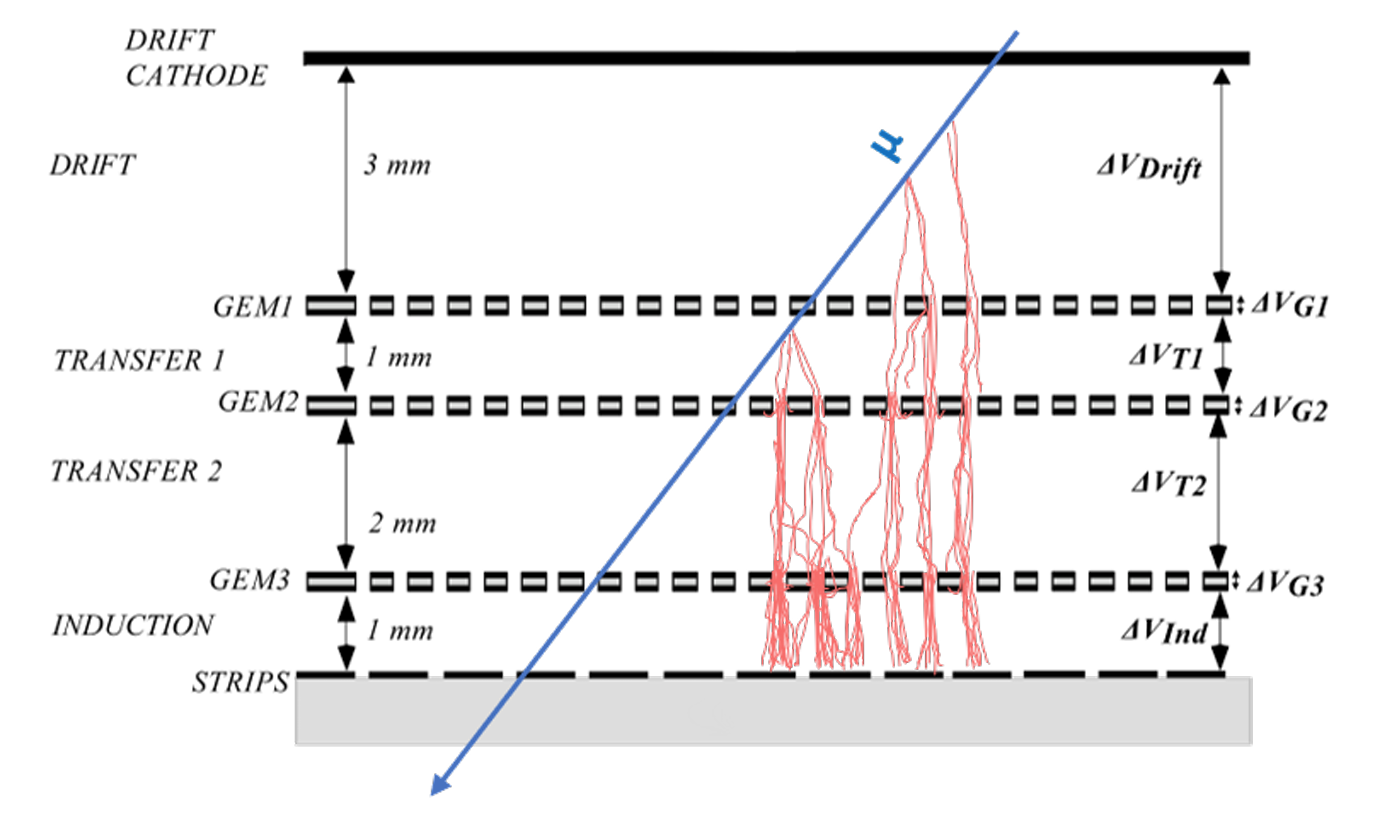
\includegraphics[width=0.8\textwidth]{Bilder/GEM_Detekro.png}
    \caption{Skizze eines Triple-Layer Gems. Das Bild wurde aus der Versuchsanleitung übernommen \cite{Anleitungsmappe}}
    \label{fig:SkizzeGem}
\end{figure}
Ein GEM (Gas-Electron-Multiplier) Detektor funktioniert in dem ein Ionisierendes Teilchen in den Detektor, bzw. um Präziser zu sein, in das Gasvolumen im Detektor eindringt und das Gas Ionisiert. Dabei werden Elektron-Ionen Paare erzeugt, die aufgrund der angelegten Spannung $V_{Drift}$ (siehe Abb. \ref{fig:SkizzeGem}) räumlich getrennt werden und nicht immer rekombinieren. Die Elektronen werden zum ersten GEM Layer beschleunigt und durch Löcher in der Kaptonfolie geleitet. In den Löchern ist die elektrische Feldstärker um die \SI{70}{\keV\per\cm^2} groß, weshalb die Elektronen auch so stark beschleunigt werden, dass sie genug Energie besitzen um weitere Gasatome zu Ionisieren. Die zurückbleibende Ionen werden zu den Kathoden, oben auf der GEM Folie beschleunigt und neutralisiert. Dieser Effekt wiederholt sich und es kommt zu einem Kaskadeneffekt. 


